\chapter{Введение}

Олимпиада Национальной технологической инициативы  (далее – Олимпиада \linebreak НТИ)\footnote{Национальная технологическая инициатива (НТИ) — это программа мер, нацеленная на формирование принципиально новых рынков и создание условий для глобального технологического лидерства России к 2035 году. Задача по созданию НТИ поставлена Президентом Российской Федерации 4 декабря 2014 года в Послании к Федеральному собранию.} – это командная инженерная олимпиада школьников, завершающаяся разработкой действующего устройства, системы устройств или компьютерной программы. Олимпиада является проектом Агентства стратегических инициатив, элементом дорожной карты НТИ «Кружковое движение» и ключевым механизмом вовлечения инженерно – ориентированных школьников в образовательные программы высшего образования, ориентированные на рынки НТИ. Оператором Олимпиады НТИ  является некоммерческая организация – Ассоциация участников технологических кружков. Профили Олимпиады НТИ выбраны на основе приоритетов Национальной технологической инициативы: «Автономные транспортные системы», «Большие данные и машинное обучение», «Системы связи и дистанционного зондирования Земли», «Интеллектуальные энергетические системы», «Нейротехнологии», «Инженерные биологические системы: агробиотехнологии и геномное редактирование», «Интеллектуальные робототехнические системы», «Беспилотные авиационные системы», «Композитные технологии», «Когнитивные технологии», «Аэрокосмические системы», «Наносистемы и наноинженерия», «Технологии беспроводной связи», «Умный город», «Передовые производственные технологии», «Виртуальная и дополненная реальность», «Анализ космических снимков и геопространственных данных», «Водные робототехнические системы» и «Программная инженерия финансовых технологий».

Цель Олимпиады НТИ: поддержка школьников в стремлении решать технологические вызовы XXI века (что подразумевает включение их в решение технологических задач переднего края и, одновременно, повышение социальной значимости такой работы старшеклассников через льготы к поступлению). Эта цель лежит в рамках большей цели Кружкового движения: формирование и подготовка команд, способных запускать глобальные технологические проекты, менять мир, создавая новые общественные практики. Именно участники этих команд должны будут через 10-15 лет «перезапустить» НТИ: создать собственные рынки и глобальные прорывные компании.  Важной особенностью олимпиады является то, что в части отборочного и в заключительном этапах участники выполняют задания в командах по 2-4 человека. Умение работать в команде - важный навык человека 21 века. Команды формируются на основе компетентностного принципа, различные компетенции участников в одной команде позволяют найти оригинальное нестандартное решение задачи.  В командах участники планируют свою работу, обсуждают, ищут совместно решения, распределяют роли - часто один участник выполняет несколько ролей. Комплексные инженерные задачи, которые решают участники, не под силу решить отдельно взятому школьнику. Задачи разработаны таким образом, что декомпозируются на несколько подзадач, за решение, которых берутся участники согласно своей роли в команде. Каждый участник несет ответственность за результат работы команды. Поэтому, при подведении итогов олимпиады определяются не только победители в личном зачете, но и команда-победитель. 

Целевыми победителями Олимпиады НТИ являются школьники, способные реализовывать сложные технические проекты в прорывных областях. Олимпиада должна выделять команды участников с особыми характеристиками мышления, коммуникации и действия, необходимыми для решения задач НТИ. Победители и призеры Олимпиады НТИ должны показывать высокие результаты в области применения предметных знаний в практической работе. Одновременно с этим, система подготовки Олимпиады НТИ должна предоставлять участникам инструменты для подготовки и получения недостающих знаний и практических навыков.

\section*{Первый год проведения олимпиады}

Олимпиада НТИ была впервые проведена в 2015/2016 учебном году. В отборочных этапах олимпиады приняли участие несколько тысяч школьников, около ста из них были приглашены к участию в заключительном этапе по профилям «Большие данные и машинное обучение», «Системы связи и дистанционного зондирования Земли», «Интеллектуальные энергетические системы», «Автономные транспортные системы». Заключительный этап Олимпиады и торжественные мероприятия проводились в ВДЦ «Орленок». 

В 2015/2016 учебном году победители и призеры олимпиады могли воспользоваться возможностью добавить дополнительные 10 баллов к сумме баллов за вступительные экзамены, в случае если они поступали в вузы-организаторы Олимпиады НТИ. 

\section*{Второй год проведения олимпиады}

В 2016/2017 учебном году Олимпиада проводилась во второй раз по 12 профилям, количество зарегистрированных для участия школьников увеличилось более чем в три раза и достигло 12 тыс., в отборочных этапах приняли активное участие 4 тыс. школьников, на заключительный этап прибыло 306 участников.  

Заключительный этап Олимпиады и торжественные мероприятия проводились на площадке Образовательного центра «Сириус», в лабораториях и помещениях Парка Наук и Искусств. Вечером проходили лекции и неформальные встречи с представителями технологических компаний. 

В 2016/2017 учебном году четыре профиля Олимпиады НТИ («Автономные транспортные системы», «Большие данные и машинное обучение», «Системы связи и дистанционного зондирования Земли», «Интеллектуальные энергетические системы») входили в Перечень олимпиад школьников, таким  образом победители и призеры смогли воспользоваться льготами при поступлении в вузы России (в зависимости от правил приема конкретного вуза). Победители и призеры новых профилей также могли воспользоваться бонусами при поступлении в вузы, которые имеют статус «организатор Олимпиады НТИ».

\section*{Третий год проведения олимпиады}

В отборе на Олимпиаду 2017/2018 учебного года приняло участие более 20 тыс. школьников, подавших более 50 тыс. заявок на различные профили, число которых увеличилось до 17. В финал вышли 578 участников Олимпиады из 51 региона РФ:

\putImgWOCaption{16cm}{history/info/map}

Финал стал распределенным и проходил с февраля по апрель 2018 года: Олимпиаду приняли Образовательный центр «Сириус», МАИ, МИФИ, ТПУ, Университет Иннополис, СПбПУ, ДВФУ, УрФУ. В 2017/2018 учебном году девять из 14 профилей Олимпиады НТИ включены в Перечень олимпиад школьников (приказ Минобрнауки России от 30.08.2017 № 866) и дают льготы при поступлении в вузы.

Важная составляющая подготовки участников к финалу Олимпиады –  открытые для всех желающих хакатоны, вебинары и мастер-классы. Программы этих мероприятий разработаны педагогами профилей Олимпиады НТИ специально для регионов так, чтобы их можно было провести на минимальном количестве оборудования. Сеть региональных партнеров Олимпиады со статусом Методическая площадка или Площадка подготовки растет с каждым годом, и в 2018 году, на третий год проведения Олимпиады, их количество достигло 110, всего проведенных мероприятий по подготовке  (соревнований, хакатонов, сборов) –  более 50. Информация о партнерских площадках размещена в специальном разделе официального сайта олимпиады: \url{http://nti-contest.ru/places_to_prepare/}.

\section*{Четвертый год проведения олимпиады}

В отборе на Олимпиаду 2018/2019 учебного года приняло участие более 36 тыс. школьников, подавших более 70 тыс. заявок на различные профили, число которых увеличилось до 19. В финал вышли 1053 участника Олимпиады из 60 регионов РФ.

Финал стал распределенным и проходил с марта по апрель 2019 года: Олимпиаду приняли МФТИ, МАИ, МИФИ, ТПУ, Университет Иннополис, СПбПУ, ДВФУ, НГУ, НовГУ, Московский Политех, ИГУ, ИРНИТУ и ряд других площадок. В 2018/2019 учебном году 13 из 19 профилей Олимпиады НТИ включены в Перечень олимпиад школьников (приказ №32н от 28 августа 2018 года Министерства науки и высшего образования Российской Федерации) и дают льготы при поступлении в вузы.

В олимпиаде в 2018/2019 учебном году впервые были проведены синхронные по времени распределенные финалы на площадках в разных городах в рамках одного профиля: Нейротехнологии (ДВФУ, НГУ, МФТИ, НовГУ), ИЭС (ИГУ, МИФИ), Нанотехнологии (Школа Летово, НГУ), АТС (Московский политех, НовГУ). Участники распределенных финалов имели одинаковые задания, критерии оценивания и единый рейтинг участников.

\section*{График проведения заключительных этапов\\Олимпиады НТИ 2018/2019 гг.}

\begin{center}
    \small
    \begin{longtable}{|p{7.5cm}|p{2.5cm}|p{5cm}|}
        \hline
        \textbf{Площадка проведения} & \textbf{Даты проведения} & \textbf{Перечень профилей Олимпиады НТИ} \\
        \hline
        \textbf{Университет Иннополис}
        
        (г. Иннополис) & 3-11 марта 2019 г. & Интеллектуальные робототехнические системы\\
        \hline
        \textbf{Университет Иннополис}
        
        (г. Иннополис) & 6-11 марта 2019 г. & Программная инженерия финансовых технологий\\
        \hline
        \textbf{Школа Летово}

        (г. Москва)

        \textbf{Новосибирский государственный университет}

        (г. Новосибирск) & 11-16 марта 2019 г. & Наносистемы и наноинженерия \\
        \hline
        \textbf{Московский политехнический университет} 

        (г. Москва) & 11-16 марта 2019 г. & Инженерные биологические системы: Агробиотехнологии \\
        \hline
        \textbf{Московский авиационный институт}

        (г. Москва) & 11-16 марта 2019 г. & Беспилотные авиационные системы \\
        \hline
        \textbf{Томский политехнический университет} 

        (г. Томск) & 12-17 марта 2019 г. & Умный город \\
        \hline
        \textbf{Иркутский национальный исследовательский технический университет}

        (г. Иркутск) & 13-19 марта 2019 г. & Технологии беспроводной связи\\
        \hline
        \textbf{Иркутский государственный университет} 

        (г. Иркутск)

        \textbf{Национальный исследовательский ядерный университет «МИФИ»}
        
        (г. Москва) & 13-19 марта 2019 г. & Интеллектуальные энергетические системы \\
        \hline
        \textbf{Иркутский государственный университет} 

        (г. Иркутск) & 13-19 марта 2019 г. & Технологии виртуальной и дополненной реальности: Дополненная реальность\\
        \hline
        \textbf{Дальневосточный федеральный университет}

        (г. Владивосток) & 18-23 марта 2019 г. & Виртуальная и дополненная реальность: Виртуальная реальность \\
        \hline
        \textbf{Дальневосточный федеральный университет} 

        (г. Владивосток) & 18-23 марта 2019 г. & Водные робототехнические системы \\
        \hline
        \textbf{Московский физико-технический институт}

        (г. Москва)

        \textbf{Новосибирский государственный университет}

        (г. Новосибирск) 

        \textbf{Новгородский государственный университет имения Ярослава Мудрого}

        (г. Великий Новгород)

        \textbf{Дальневосточный федеральный университет}

        (г. Владивосток) & 18-23 марта 2019 г. & Нейротехнологии \\
        \hline 
        \textbf{Московский физико-технический институт}

        (г. Москва),

        \textbf{Новосибирский государственный университет}

        (г. Новосибирск) & 18-23 марта 2019 г. & Инженерные биологические системы: Геномное редактирование \\
        \hline
        \textbf{Московский физико-технический институт}

        (г. Москва) & 18-23 марта 2019 г. & Большие данные и машинное обучение \\
        \hline
        \textbf{АО «ИПК Машприбор» ГК Роскосмос} 

        (г. Королев)

        \textbf{Детский технопарк «Кванториум»}

        (г. Королев) & 26-31 марта 2019 г. & Системы связи и дистанционного зондирования Земли \\
        \hline
        \textbf{АО «ИПК Машприбор» ГК Роскосмос}

        (г. Королев)

        \textbf{Детский технопарк «Кванториум»}

        (г. Королев) & 26-31 марта 2019 г. & Аэрокосмические технологии \\
        \hline
        \textbf{АО «ИПК Машприбор» ГК Роскосмос}

        (г. Королев)

        \textbf{Детский технопарк «Кванториум»}

        (г. Королев) & 26-31 марта 2019 г. & Анализ космических снимков и пространственных геоданных Земли \\
        \hline
        \textbf{Санкт-Петербургский университет Петра Великого,}

        \textbf{Академия цифровых технологий}

        (г. Санкт-Петербург) & 01-06 апреля 2019 г.	& Передовые производственные технологии \\
        \hline
        \textbf{Московский государственный психолого-педагогический университет}
        
        (г. Москва) & 02-06 апреля 2019 г. & Когнитивные технологии \\
        \hline
        \textbf{Московский государственный технический университет им. Н.Э. Баумана}

        (г. Москва) & 07-12 апреля 2019 г. & Композитные технологии \\
        \hline
        \textbf{Московский политехнический университет}
        (г. Москва)

        \textbf{Новгородский государственный университет имения Ярослава Мудрого}

        (г. Великий Новгород) & 08-14 апреля 2019 г. & Автономные транспортные системы\\
        \hline        
    \end{longtable}
\end{center}

\section*{Организаторы и партнеры Олимпиады НТИ}

Оргкомитет олимпиады представлен ректорами крупнейших политехнических и инженерных вузов России, руководителями технологических компаний и представителями государственных органов.

\textbf{Вузы-соучредители олимпиады:}
\begin{itemize}
    \item ФГБОУ ВО «Московский политехнический университет»;
    \item ФГАОУ ВО «Санкт-Петербургский политехнический университет Петра Великого»;
    \item ФГАОУ ВО «Национальный исследовательский Томский политехнический университет»;
    \item ФГАОУ ВО «Дальневосточный федеральный университет».
\end{itemize}

\textbf{Технологические партнеры}

Олимпиада НТИ проводится при поддержке технологических партнеров, количество которых увеличилось, по сравнению с прошлым годом,  среди них: РВК (Российская венчурная компания) и АСИ (Агентство стратегических инициатив по продвижению новых проектов)  –  в роли со-организаторов и генеральных партнеров выступают: Аэрофлот, ПАО «Сухой», ОАК, Роскосмос, ФИОП Роснано, МТС, Газпром нефть, Фонд новых форм развития образования, сеть детских технопарков «Кванториум», Спутникс, Полюс-НТ, BiTronicsLab, КРОК,  Инфосистемы Джет, Лоретт, Коптер Экспресс, АсРоботикс, Образование будущего и др. Полный список организаторов и партнеров олимпиады размещен в соответствующем разделе на официальном сайте: \url{http://nti-contest.ru/about/}.

\textbf{Вузы-организаторы профилей Олимпиады НТИ:}
\begin{itemize}
    \item АНО ВО «Университет Иннополис»; 
    \item ФГАОУ ВО «Национальный исследовательский ядерный университет «МИФИ»;
    \item ФГАОУ ВО «Московский физико-технический институт (государственный университет)»;
    \item ФГБОУ ВО «Московский авиационный институт (национальный исследовательский университет)»;
    \item ФГБОУ ВО «Сибирский государственный университет науки и технологий имени академика М.Ф. Решетнева»;
    \item ФГАОУ ВО «Новосибирский национальный исследовательский государственный университет»;
    \item АНО ВО «Сколковский институт науки и технологий»;
    \item ФГБОУ ВО «Московский государственный психолого-педагогический университет»;
    \item ФГБОУ ВО «Московский государственный технический университет имени Н.Э. Баумана (национальный исследовательский университет)»;
    \item ФГБОУ ВО «Новгородский государственный университет имени Ярослава Мудрого»;
    \item ФГБОУ ВО «Иркутский государственный университет»;
    \item ФГБОУ ВО «Новосибирский государственный технический университет»;
    \item ФГАОУ ВО «Национальный исследовательский Нижегородский государственный университет им. Н.И. Лобачевского»;
    \item ФГБОУ ВО «Московский технический университет связи и информатики».
\end{itemize}

К работе методической комиссии был привлечен профессорско-преподавательский состав вузов-организаторов и представители реального сектора экономики. Объективную оценку работы осуществляет жюри, представленное основателями технологических компаний, а также представителями вузов-организаторов.  

Вузы-организаторы, входящие в Оргкомитет Олимпиады НТИ, ведут непрерывную работу с талантливыми школьниками.

\textbf{ООО Полюс-НТ и ООО ИнСитиЛаб} являются организаторами профиля «Технологии беспроводной связи».

Компании являются ведущими разработчиками образовательных продуктов и программ для научно-технического творчества детей и молодежи. Область деятельности: современное естествознание и нанотехнологии; интеллектуальная энергетика, кибербезопасность и технологии беспроводной связи. 

Кроме коммерческих проектов компании специализируется на создании «Нового образовательного пространства», которое объединяет образовательные занятия и мероприятия (конференции, проектные школы, курсы повышения квалификации, семинары) для детей и взрослых, и направлено на развитие культуры проектной деятельности и STEM-формата обучения. Компании являются разработчиками треков Всероссийских мероприятий, направленных на развитие научно-технического творчества молодежи – Олимпиады НТИ, Всероссийских проектных школ, образовательных интенсивов.
\begin{itemize}
    \item С 2010 года компания Полюс-НТ является организатором мероприятий различного уровня в области проектной деятельности школьников (Открытая научно-практическая конференция для школьников и студентов в области естествознания и инновационных технологий «Удивительный мир», 2011-2019 гг, Всероссийская летняя школа-конференция «Проектное образовательное пространство в области естествознания и нанотехнологий», 2011, 2012, 2013, 2014, 2015). Соорганизатором Всероссийских мероприятий (ряда проектных школ под эгидой «Лифт в будущее», «Иннопрактика», Intel, Всероссийских мероприятий под эгидой Кружкового движения НТИ).
    \item С 2015 года компания Полюс-НТ открыла ЦМИТ «STEM-Байкал» – площадку для развития в области научно-инженерного творчества молодежи, на которой проводятся регулярные занятия и мероприятия для школьников и студентов.
    \item 2015, 2016 годы. Представление стенда «Интеллектуальные энергетические системы» на Всероссийском форуме «Будущие интеллектуальные лидеры России»
    \item В 2016 году компания Полюс-НТ вошла в национальный реестр как Ведущая научная организация России
    \item С 2016 года компания «Полюс-НТ» является разработчиком трека первой инженерной Олимпиады НТИ «Интеллектуальные энергетические системы». С 2017 года разработчиком второго трека «Технологии беспроводной связи». С 2018 года компания ИнСитиЛаб стала разработчиком трека «Технологии беспроводной связи»
    \item С 2017 года компания Полюс-НТ является методической площадкой для подготовки к Олимпиаде НТИ в Иркутской области.
    \item В 2017 году компания Полюс-НТ стала финалистом конкурса Мосгортех 2017 с проектом Междисциплинарный практикум по естествознанию и нанотехнологиям «Нанолаб».
    \item В 2018 год компания Полюс-НТ вошла в число организаторов образовательного интенсива для технологических лидеров Остров 10–21. Проведены две лаборатории: Лаборатория интеллектуальной энергетики; AR-лаборатория для создания упаковки настольных игр.
    \item В 2018 году Проект «Игротека НТИ», реализуемый с сентября 2017 года в ЦМИТ под руководством нашего волонтера Алены Просекиной (выпускницы МБОУ Лицей №2 и ученицы многих образовательных курсов от наших педагогов), занял II место на Всероссийском конкурсе лучших практик наставничества «Наставник — 2018» в номинации «Дети учат детей».
\end{itemize}

Компании активно работают со школьными учителями и педагогами дополнительного образования, организуются курсы подготовки для педагогов и наставников.
\begin{itemize}
    \item Компанией Полюс-НТ проведены неоднократно Курсы повышения квалификации «Изучение нанотехнологий в школе, как основа внедрения междисциплинарного и проектного подхода», 2014; Курсы повышения квалификации «Основы проектной деятельности в области естествознания и нанотехнологий», лето 2012, 2013, 2014, 2015, Международная конференция «Нанотехнологии в образовании», 2014)
    \item В 2018 году компаниями организованы и проведены Образовательный интенсив для наставников по тематикам и кросс-отраслевым технологиям НТИ, а также Островной десант в Иркутске: мини-интенсив от экспертов НТИ и преподавателей Острова.
\end{itemize}

Вузы-организаторы, входящие в Оргкомитет Олимпиады НТИ, ведут непрерывную работу с талантливыми школьниками.
    
\textbf{Московский политехнический университет}

Московский политехнический университет при активном участии Инженерной школы (факультета) регулярно ведет мероприятия для школьников. Факультет «Инженерная школа» создан в 2016 году в целях развития работы Московского Политеха с детьми старшего школьного возраста и организации участия университета во всероссийских и региональных программах по поддержке талантливых школьников.

Факультет курирует проекты Департамента образования г. Москвы «Центр технологической поддержки образования» (с 2013 года) и «Инженерный класс в московской школе» (с 2015 года) в целях повышения количества выпускников московских школ, поступивших в инженерные вузы столицы. В 2017 году под научно-методическим руководством сотрудников факультета открыты инженерные классы в 41 школе города Москвы (более 3000 учащихся 10-11 классов). Преподаватели инженерной школы ведут занятия в технологических кружках на базе Московского Политеха, курсы повышения квалификации для преподавателей московских школ, организуют инженерные соревнования и профориентационные мероприятия: экскурсии на предприятия, встречи с носителями профессионального опыта, инженерные турниры и соревнования.

Для подготовки учащихся к инженерной проектной деятельности и вовлечения их в техническое творчество Инженерная школа с октября 2016 года открыла кружки для старшеклассников (8-11 класс):
\begin{itemize}
    \item Космическая инженерия;
    \item Кружок схемотехники и микроэлектроники;
    \item Техника низких температур;
    \item Инфракрасные технологии и радиоэлектроника;
    \item Программирование на С++;
    \item Аквапонные системы;
    \item Автомобилестроение;
    \item Беспилотный транспорт;
    \item Кружок 3D моделирования и прототипирования и другие.
\end{itemize}

Важнейшим направлением работы факультета является организация выездных инженерных школ и профильных смен, попасть на которые имеют возможность дети из любых регионов России, проявившие уникальные способности в научно-технической сфере.

Образовательный центр «Сириус» и Московский политехнический университет являются официальными партнерами. Летом 2016 года Московский Политех выступил соорганизатором трех направлений проектной деятельности в ОЦ «Сириус» и осуществил экспертную поддержку деятельности центра по направлениям «Транспорт» и «Космос». В июле 2017 года Московский Политех стал соорганизатором направления «Наука», в котором приняли участие 400 учеников 8-10 классов, прошедшие конкурсный отбор. Преподаватели и студенты университета приняли участие в организации направлений «Беспилотный транспорт и логистические системы», «Спутники и пилотируемая космонавтика», «Персонализированная медицина» и «Современная энергетика». В планах факультета - создание инженерных кружков Московского Политеха на базе Сириуса (радиотехника, аэрокосмическая инженерия) и лаборатория беспилотного транспорта.

С 2016 года факультет организует участие Московского Политеха в ежегодном форуме талантливых детей «Проектория» в г. Ярославле. Форум проводится под руководством аппарата полномочного представителя Президента Российской Федерации в ЦФО и Министерства образования и науки Российской Федерации. В форуме принимают участие до 500 школьников со всей страны. В ноябре 2016 года и сентябре 2017 года Московский Политех выступил партнером образовательной программы форума в рамках направления «Технологии движения». В ноябре 2018 года Московский Политех принимал участие в фестивале “Билет в будущее” в рамках направлений “Космос”, “Транспорт”, “Новые материалы”, “Умная среда”.

С 2016 года Инженерная школа (факультет) является соорганизатором и партнером инженерно-конструкторских школ «Лифт в будущее» - программа БФ «Система» по поддержке талантливой молодежи. В течение октября 2017 года вместе с преподавателями Московского Политеха в ВДЦ «Орленок» дети разрабатывали технологические проекты, две из восьми лабораторий курировали сотрудники и студенты университета.

В январе 2018 года, июне 2018 года, октябре 2018 года и феврале 2019 года совместно с Центром педагогического мастерства (Департамент образования гор. Москвы) факультет провел выездную инженерную школу Московского Политеха для учащихся инженерных классов города Москвы, приняли участие 160 человек.

В марте 2018 года поддержке Департамента науки, промышленной политики и предпринимательства города Москвы в Московском Политехе открылся детский технопарк Центра развития инжиниринга - инженерно-технологический комплекс, на базе которого проводятся углубленные технико-ориентированные курсы дополнительного образования для школьников. На данный момент запущены 4 образовательных программы: Транспортный дизайн, Введение в автомобилестроение, Беспилотный транспорт и Современная космонавтика.

Вместе с тем Московский Политех принимает участие в организации других олимпиад, входящих в перечень олимпиад школьников Минобрнауки России:
\begin{enumerate}
    \item Объединенная межвузовская математическая олимпиада (ОММО). Проводится для одиннадцатиклассников по инициативе группы московских вузов с 2009 года.
    \item Международная олимпиада школьников «Искусство графики». Проводится с целью выявления и привлечения наиболее подготовленных, талантливых и профессионально ориентированных учащихся средних художественных училищ РФ и ближнего зарубежья, школьников, слушателей подготовительных курсов, развитие у обучающихся творческих способностей, содействие профессиональной ориентации школьников.
\end{enumerate}

Московский Политех также участвует (имеет статус организатора или со-\linebreak организатора) в следующих мероприятиях: инженерно-конструкторское направление предпрофессиональной олимпиады Московской олимпиады школьников 2016-19~гг., предпрофессиональный экзамен для инженерных классов в Москве 2016-2019~гг., инженерное направление Московского конкурса научно-исследовательских и проектных работ учащихся, проектные смены ОЦ «Сириус», турнир двух столиц по робототехнике и т.д.

\textbf{Санкт-Петербургский политехнический университет Петра Великого}

В 2010 году получил статус национального исследовательского университета, что явилось признанием его роли и возможностей как в области подготовки кадров, так и в мультидисциплинарных научных исследованиях и разработках. В рейтинге технических университетов России Политехнический неизменно занимает ведущие позиции.

СПбПУ активно работает со школьниками со всей страны. В ВУЗе работает Центр профориентации и довузовской подготовки, где учащиеся могут получить дополнительные знания по школьным предметам основного образования. Также активную работу со школьниками ведет Центр научно-технического творчества молодежи Фаблаб Политех.

В рамках довузовской подготовки в Университете успешно функционируют такие проекты, как «Вызов Политехника», «Мой город цифровой» и проектные интенсивы для школьников от Фаблаб Политех, где более 3 000 учащихся проходят обучение по передовым направлениям дополнительного образования. Подшефные школьники ежегодно демонстрируют высокие результаты на Всероссийских и международных конкурсах для молодых профессионалов: WorldSkills, Реактор, Олимпиада НТИ, Техномейкер, Шустрик, Кубок ЦНИИ РТК. Университет активно работает со школьными учителями и педагогами дополнительного образования, организуются курсы повышения квалификации для педагогов по программам дополнительного образования, проводятся собственные конкурсы для учащихся и педагогические конференции.

\textbf{Томский политехнический университет}

Сегодня ТПУ – опорный вуз для крупнейших государственных корпораций, среди которых «Газпром», «Росатом», АО «”Информационные спутниковые системы” имени академика М.Ф. Решетнева», «Микроген», «Системный оператор ЕЭС», «РАО Энергетические системы Востока».

В 2009 году в ТПУ был запущен Интернет-лицей, позволяющий школьникам подготовиться к вступительным испытаниям в режиме онлайн.

Для школьников и их учителей, занимающихся исследовательской работой, мы проводим ежегодные конференции. Это - Всероссийская конференция-конкурс исследовательских работ старшеклассников «Юные исследователи - российской науке и технике», Межрегиональная научно-практическая конференция для учителей «Организация исследовательской деятельности детей и молодежи: проблемы, поиск, решения»,  конкурс учителей физики «От школьной физики – к высоким технологиям» и конкурс учителей химии «Мой выбор – химия».

Лицей при Томском политехническом университете создан в 1992 г. Лицей имеет физико-математический профиль и полностью располагается на площадях университета. В  2015 г.  в Лицее при ТПУ открыт первый в Сибири профильный класс компании «Газпром». По результатам итоговой аттестации в форме ЕГЭ  лицей занимает лидирующие позиции в регионе, демонстрируя при этом постоянную положительную динамику. Лицей при ТПУ входит  в ТОП-10  рейтинга лучших школ по качеству подготовки к поступлению в ведущие высшие учебные заведения России и топ-500 лучших школ России по результатам рейтинга, составленного Московским центром непрерывного математического образования. Все выпускники лицея ТПУ поступают в вузы. Лицеисты – постоянные участники и дипломанты Международных научно-технических конференций школьников, проводимых МГУ, МФТИ, НИЯУ МИФИ и др.

\textbf{Дальневосточный федеральный университет} (г. Владивосток) – один из крупнейших университетов на Дальнем Востоке России.

Дальневосточный федеральный университет уделяет большое внимание привлечению абитуриентов со всей страны, выявлению и поддержке талантливых школьников в области инженерных и естественных наук.
\begin{enumerate}
    \item Олимпиады. Дальневосточный федеральный университет проводит три собственные олимпиады:
    \begin{itemize}
        \item «Океан знаний». Предметы: математика, физика, химия, биология, география, русский язык, литература, история и обществознание.
        \item «Ближе к Дальнему». Предметы: история (включая культурологию), география (включая экономику), биология, филология (включая литературу и лингвистику), международные отношения и политология.
        \item «Турнир юных программистов». Предметы: программирование.
    \end{itemize}

    В 2018/2019 году ДВФУ стал площадкой для Всероссийских олимпиад:
    \begin{itemize}
        \item Олимпиада Национальной технологической инициативы (НТИ)
        \item Всероссийская олимпиада школьников (региональный этап)
        \item Евразийская лингвистическая олимпиада
        \item Физико-математическая олимпиада «Физтех»
        \item Всероссийская командная школьная олимпиада по программированию
        \item Северо-Восточная олимпиада школьников
        \item Объединенная межвузовская олимпиада по математике
        \item Открытая олимпиада по экономике
        \item Олимпиада для школьников «Ломоносов»
        \item Объединённая межвузовская математическая олимпиада
        \item Олимпиада СПбГУ
        \item Математическая олимпиада им. В.Б. Осипова 
    \end{itemize}

    С 2012 года в рамках смены «Российский интеллект» реализуется совместная образовательная программа Дальневосточного федерального университета и Всероссийского детского центра «Океан» для победителей и призеров региональных этапов Всероссийской олимпиады школьников и победителей/призеров отборочного этапа олимпиады школьников «Океан знаний».
    \item Проекты дополнительного образования для талантливых школьников:
    \begin{itemize}
        \item «Тихоокеанские Школы ДВФУ»: учебно-тренировочные сборы. Проводятся по предметам: математика, программирование, английский язык, китайский язык. В год на базе ДВФУ проходит 4 сессии, когда школьники на неделю погружаются в интенсивное изучение предмета. В 2017/2018  годах в «Тихоокеанских школах ДВФУ» приняли участие более 700 школьников, 140 преподавателей прошли курсы повышения квалификации.
        \item «Тихоокеанская проектная школа». Совместный образовательный проект Дальневосточного федерального университета и Всероссийского детского центра «Океан».Для участия в конкурсном отборе необходимо подать заявку с идеей по развитию Дальнего Востока.Участниками «Тихоокеанской проектной школы» в июне-июле 2017 года стали 100 старшеклассников в возрасте 15-17 лет. За три недели они подготовили проекты по четырем направлениям:инженерное,естественно-научное, социально-гуманитарное и современные информационные технологии. Авторы лучших проектов представили свои разработки на III Восточном экономическом форуме, который прошел в ДВФУ в сентябре 2017 г.
        \item Образовательная программа «Яндекс.Лицей». Проект стартовал на базе ДВФУ в 2017 году. Ученики 8–9 классов дважды в неделю осваивают программирование на языке Python. Для лицеистов ДВФУ проводит «Хакатон» – трехдневное интенсивное погружение в предмет.  Обучение бесплатное. Поступление на конкурсной основе. В 2018/2019 учебном году ДВФУ планирует вдвое увеличить количество учеников «Яндекс.Лицея».
        \item Роснефть классы. Роснефть-класс – профильный класс, сформированный в результате конкурсного отбора учащихся, обучающихся по углубленным программам физики, математики, информатики, ориентированный на выбор профессий, связанных с судоремонтом и судостроением.
        \item JUNIOR РОСТ. Программа бизнес-школы «JUNIOR РОСТ» направлена на развитие способностей предпринимательства у школьников от зарождения предпринимательской идеи до реализации, организации совместных проектных групп из обучающихся и представителей бизнес-среды, получению дополнительных знаний из других областей, нахождению единомышленников. Данное направление апробировано в 2018 году в рамках Русско-азиатской бизнес-школы «РОСТ».
        \item Взаимодействие с Образовательным центром «Сириус». «Социальный лифт» – организация и проведение региональных треков Всероссийских мероприятий Образовательного центра «Сириус». Обеспечение раннего выявления, развития и дальнейшая профессиональная поддержка одаренных детей, проявивших выдающиеся способности в к проектной, научной (научно-исследовательской), инженерно-технической, изобретательской, творческой деятельности.
        \item Кадры будущего. Проект направлен на поддержку талантливых школьников и студентов, неравнодушных к судьбе Приморского края и готовых включиться в реализацию проектов в важных для региона социально-экономических направлениях развития.В рамках проекта участникам будет предоставлена возможность разработать проект, а также пройти стажировку на предприятиях в разных отраслях экономики: транспорт и логистика, машиностроение и судоремонт, рыбная промышленность, сельское хозяйство и пищевая промышленность, сервис и туризм, строительство и умный город, экология и марикультура.
    \end{itemize}
\end{enumerate}

\section*{Структура отбора участников Олимпиады НТИ}

Соревнование проходит в три этапа. Первый и второй отборочные этапы проходили с октября по декабрь 2018 года в заочной форме на интернет-платформе «Stepik» (\url{http://stepik.org}) и в инженерных онлайн-симуляторах.

Отборочные этапы сопровождались различными подготовительными мероприятиями, среди которых были дистанционные мероприятия (вебинары), мероприятия для самостоятельной подготовки (онлайн-курсы), мероприятия направленные на командообразующую деятельность (специальные встречи, интенсивы, очные курсы на площадках по подготовке, создана специальная интерактивная форма формирования и подбора членов команд на платформе Олимпиады НТИ), мероприятия, направленные на получение практических навыков (интенсивы).

Заключительный этап Олимпиады состоит из двух частей: индивидуальное решение предметных задач по выбранным профилям и командная разработка инженерного решения с испытанием  его на стенде. Задание второй части заключительного этапа имеет свою специфику для каждого профиля.

\section*{Информация о профиле}

Задачи на профиле связаны с актуальными задачами систем связи, включая вопросы помехоустойчивого кодирования, передачи информации в условиях шумов, работы с различными форматами данных, разработки адаптивной системы слежения и т.д. Ключевые области применения связаны с космосом, промышленным интернетом вещей, подводной и мобильной робототехникой, каналами связи для роевых устройств. В ходе командного финала командам предстоит решать взаимосвязанные задачи, связанные с помехоустойчивым кодированием и декодированием, передачей данных  по каналам с различной зашумленностью и скоростью, алгоритмами слежения за объектом с частично детерминированной траекторией. Для этого участникам будет необходимо разобраться с физическими свойствами закодированного сигнала, программными алгоритмами разбиения данных на блоки с различной избыточностью кодирования для различных каналов, а также с восстановлением по данным физического моделирования траекторной информации и диаграммы направленности. 

\putImgWOCaption{10cm}{history/info/telecom/1}

\begin{center}
    На фото: Участники профиля «Технологии беспроводной связи» за работой
\end{center}

\section*{Работа с участниками}

Организаторы Олимпиады заинтересованы в дальнейшем сопровождении ее участников. Практика показывает, что школьники  –  участники Олимпиады НТИ также заинтересованы в дальнейшем сотрудничестве. В организации заключительного этапа Олимпиады НТИ 2018/2019 учебного года в качестве волонтеров приняли участие победители и призеры Олимпиады НТИ 2017/2018 учебного года, студенты первых курсов из различных регионов России. Участники заключительного этапа 2018/2019 учебного года из числа учеников одиннадцатого класса также выразили желание принять участие в организации олимпиады и подготовке участников в качестве волонтеров.  

В 2018/2019 годах число партнерских мероприятий Олимпиады увеличилось: на странице \url{http://nti-contest.ru/participants/posle_finala/} представлен список мероприятий, организаторы которых специально приглашают участников Олимпиады и дают им бонусы при конкурсном отборе.

Так, члены команд-победителей финалов Олимпиады были приглашены на образовательный интенсив «Остров 10-22», проходящий в Сколково летом 2019 года.  На авиационную смену в «Артеке» получили приглашение лучшие участники профиля «Беспилотные авиационные системы». Отбор на июльскую проектную смену в Образовательный центр «Сириус» предполагает дополнительные баллы для призеров и победителей Олимпиады НТИ.

\section*{Партнерство с инженерными соревнованиями}

Оргкомитет Олимпиады НТИ, в свою очередь, ежегодно утверждает перечень инженерных мероприятий и конкурсов, победители которых, могут принять участие в заключительном этапе Олимпиады, минуя отборочные. В 2016/2017 учебном году таковыми мероприятиями являлись: IT-хакатон GoTo, инженерно-конструкторские школы «Лифт в будущее»,  всероссийский форум «Будущие интеллектуальные лидеры России» и World Skills High Tech. 

В 2017/2018 учебном году льготы предоставлялись победителям мероприятий: всероссийский форум «Будущие интеллектуальные лидеры России», чемпионат \linebreak «WorldSkills Abu Dhabi» и «World Skills High Tech (Junior)», Воздушно-инженерная школа МГУ, региональный этап международных соревнований по подводной робототехнике «Russia Far-East MATE ROV Competition», Всероссийская Робототехническая Олимпиада.

В 2018/2019 году напрямую во второй этап Олимпиады получили доступ победители Региональных чемпионатов WorldSkills Junior Russia, Всероссийской робототехнической олимпиады, Олимпиады «Шаг в Будущее», Russia Far-East MATE ROV Competition, Russian Self-Driving Challenge, трека «Микробный топливный элемент» конкурса icet2018.ru, конкурса «Энергопрорыв» 2017/2018, Всероссийской олимпиады по 3D технологиям «Робофинист», Олимпиада «Кибервызов» компании Ростелеком, проектных смен Образовательного центра «Сириус» и всероссийских олимпиад школьников 1-3 уровней.

\section*{Равные возможности для участников с  ограниченными возможностями здоровья}

Организаторы Олимпиады НТИ соблюдают принцип равных возможностей и доступности участия школьников с ограниченными возможностями здоровья. В Олимпиаде беспрепятственно могут участвовать школьники с с ограниченными возможностями здоровья, обучающиеся дети-инвалиды, а также те, кто обучался по состоянию здоровья на дому. Важное условие для участия в олимпиаде детей с ОВЗ и инвалидностью - способность выполнять инженерные работы и работать в команде.

\putImgWOCaption{10cm}{history/info/telecom/i1}

Отборочные этапы олимпиады проводятся дистанционно, это позволяет детям 7-11 классов с ОВЗ и инвалидам решать задания в домашних условиях или в образовательной организации, оборудованной с учетом их индивидуальных особенностей.

Для проведения заключительного этапа соревнований были выбраны площадки с соответствующими материально-техническими условиями, которые обеспечивают: возможность беспрепятственного доступа участников олимпиады в аудитории, туалетные и иные помещения, а также их пребывания в указанных помещениях; наличие пандусов, поручней, расширенных дверных проемов, лифтов, при отсутствии лифтов аудитория располагается на первом этаже наличие специальных кресел и других приспособлений. 

\begin{figure}[H]
    \begin{center}
    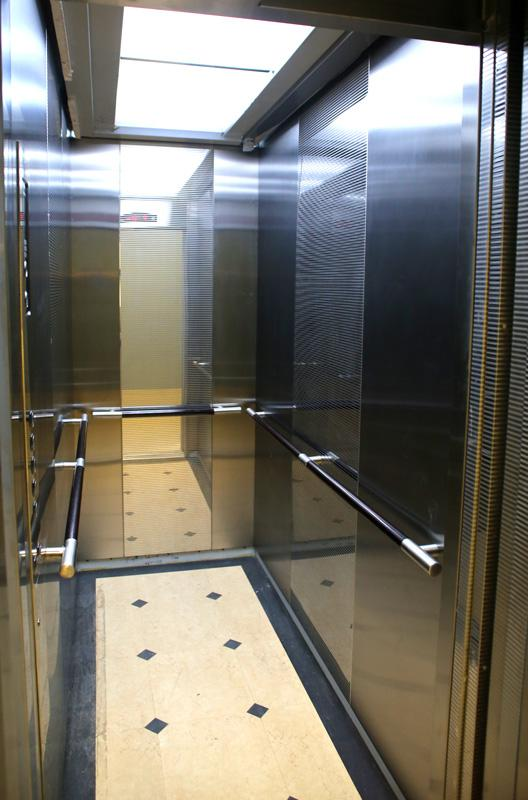
\includegraphics[width=5cm]{history/info/telecom/i2}
    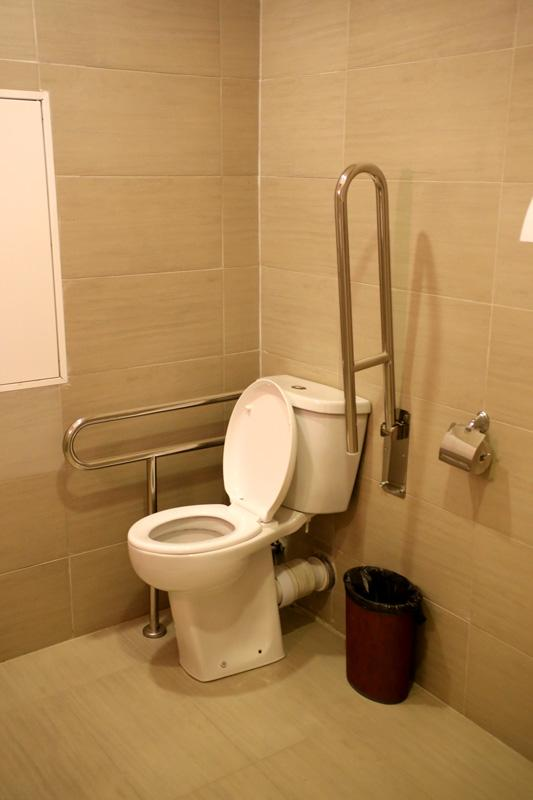
\includegraphics[width=5cm]{history/info/telecom/i3}
\end{center}
\end{figure}

Большинство площадок проведения финалов олимпиады оснащены паспортами доступности для инвалидов объектов и предоставляемых в этих объектах услуг.

\putImgWOCaption{10cm}{history/info/telecom/i4}

При проведении олимпиады в случае необходимости возможно сопровождение детей с ОВЗ ассистентами (сопровождающие лица или родители), оказывающими участникам с ОВЗ, детям-инвалидам и инвалидам необходимую техническую помощь с учетом их индивидуальных особенностей, помогающими им занять рабочее место, передвигаться, прочитать задания. 

В заключительных этапах олимпиады 2018/2019 учебного года приняло участие 9 школьников с ОВЗ, для которых были созданы все необходимые условия для полноценной работы и своевременного оказания необходимой медицинской и иной помощи. Во время проведения олимпиады сопровождающие могли сделать экспресс-анализ крови, дать при необходимости лекарство, сделать укол. На каждой площадке проведения олимпиады находился дежурный врач, который оказывал необходимую медицинскую помощь в т.ч. и детям с ОВЗ.

\putImgWOCaption{10cm}{history/info/telecom/i5}

\section*{Подготовка участников}

Для вовлечения участников в олимпиаду были разработаны «Урок НТИ» и «Демо-этап» олимпиады, благодаря чему участники могли определиться с выбором профилей и попробовать свои силы.

«Урок НТИ» (\url{http://nti-contest.ru/ntilessonteacher/}) – это инициатива Олимпиады НТИ, проходившая в сентябре 2018 года и направленная на распространение информации об НТИ среди школьников и привлечение их к Олимпиаде НТИ через проведение уроков и занятий в школах и учреждениях дополнительного образования. Учебный материал для проведения «Урока НТИ» сформирован в виде конструктора, с помощью которого учителя могли собрать урок по теме НТИ. Урок позволяет познакомить учащихся НТИ и  с профилями Олимпиады НТИ, организовать практическую работу по решению задач в рамках выбранного профиля. Для участия в проекте «Урок НТИ» зарегистрировалось 2185 педагогов.

Демо-этап Олимпиады НТИ (\url{https://stepik.org/course/24389/syllabus}) – это публикация задач олимпиады в открытом доступе. Демо-этап создан для знакомства с задачами по профилям олимпиады, тренировки и испытания собственных знаний и умений решать непростые инженерные задачи.  Прежде чем определиться с участием в олимпиаде и выбором профиля,  потенциальные участники и их наставники могут познакомиться с задачами и выбрать наиболее интересный для себя профиль.

Чтобы участники могли восполнить недостаток практических компетенций и изучить оборудование, на котором им предстоит работать на заключительном этапе Олимпиады НТИ, разработчики направлений представляют методические материалы для самостоятельной практики и самоподготовки, проводят вебинары для участников и педагогов с ответами на вопросы и подбирают подготовительные курсы, совместно с площадками подготовки проводят хакатоны для участников с возможностью попробовать на практике фрагменты финальной задачи. 

Команды разработчиков профилей с целью эффективной подготовки к Олимпиаде НТИ создали видео разборы задач 2 этапа, которые доступны на канале Олимпиады НТИ, \url{https://www.youtube.com/channel/UCZV1CNpOrDNj7tuWuf35lgw/playlists} в 2018 году разработан курс (веб-сайт: \url{https://stepik.org/course/15697/syllabus}) по подготовке школьников к Олимпиаде НТИ на основе контента олимпиады 2017/2018 учебного года. Курс содержит задачи предметных треков 1 и 3 этапа по предметам: математика, физика, информатика, химия и биология и задачи 2 этапа по профилям олимпиады. Курс может использоваться наставниками и самими участниками для подготовки к олимпиаде следующего года. Формат курса максимально приближает участников к реальным условиям олимпиады.

Все указанные материалы находятся в свободном доступе и размещены на официальном сайте олимпиады, на страницах профилей в разделе «Материалы для участников». 

Материалы по профилю «Технологии беспроводной связи»: \url{http://nti-contest.ru/profiles/telecom/}

Олимпиада НТИ является промежуточным итогом работы по реализации дорожной карты НТИ «Кружковое движение»: подготовка к ней велась в фаблабах, ЦМИТах, детских технопарках, на базе активных школ и лицеев, центров дополнительного образования по всей России. Рабочая группа «Кружковое движение» НТИ направлена на развитие технологического сообщества, объединяющего школьников и студентов, ориентированных на инженерную деятельность на рынках НТИ, самодеятельных технических энтузиастов, лидеров технологических кружков, разработчиков педагогических технологий, технологических предпринимателей, популяризаторов науки и технологий.

\section*{Популяризация Олимпиады НТИ}

Олимпиада НТИ широко освещается в различных средствах массовой информации (телевидение, печатные издания, электронные издания). В период с 15 августа 2018 года (начало подготовки к регистрациям) до 3 апреля 2019 года, по данным Медиалогии, Олимпиада НТИ упоминалась в СМИ 2 301 раз, из них 633 раза на федеральном уровне, 1655 на региональном уровне, 13 на зарубежном уровне. 

Во время проведения отборочных этапов Олимпиада НТИ освещалась в федеральных, массовых, родительских, образовательных и иных медиа («ИТАР-ТАСС», «РИА-Новости», «Интерфакс», «Такие Дела», «Летидор», «Дети.Мэйл.ру», «Индикатор», «Занимательная робототехника», «Чердак.Ру», «Habrahabr», «Rusbase», \linebreak «Учёба.Ру»), официальных образовательных порталах и порталах органов государственности власти в регионах  (Новосибирск, Санкт-Петербург, Великий Новгород, Иннополис, Томск, Владивосток, Калининград, Тюмень, Курск, Курган, Тамбов, Мурманск, Новогород, Вологда и т.д.), в печатных изданиях («Российская газета», «Известия»). Радио «Медиаметрикс», программа «Выбор Родителей» под руководством автора самого большого блога для родителей в России.  Кампания по привлечению шла также в научно-популярных группах и группах вузов и площадок партнеров (МАИ, НГУ, Абитуриент НГУ,  ДВФУ, Школьники ДВФУ, Абитуриенты ДВФУ, Мурманский Арктический государственный университет, СибГУ им. М.Ф. Решетнева, Кванториум, АНО ДТ Красноярский кванториум,  НовГУ, ТПУ, абитуриенты ТПУ, МГППУ, Московский Политех, школа Летово, технопарк Академгородка, Сколтех, Иннополис, группы довузовского управления университета Иннополис, Политех Петра, ИТМО, ИРНИТУ, студенты ИРНИТУ, АУ УР РЦИиОКО, Детский технопарк INGENERIKA, Инкубатор Профи, Центр компетенций для детей Поколение 2035, Лаборатория НГУ Инжевика, Чеченский государственный университет, Айти школа Орбита, Фонд Книту, Фонд Золотое сечение, ЦМИТЫ Коптер, Ноосфера, Рекорд, Уникум, Stem-Байкал, Роболатория, Академия Технолаб, Образовательный проект для подростков Tula Teens ,  Проектория, ЯКласс, Фаблаб Политех и другие).  Заключительный этап Олимпиады НТИ в 2018/2019 учебном году проходил при участии журналистов таких печатных изданий, как «Российская газета», «Известия»; федеральных телевизионных каналов («Россия 24» (6 репортажей), «Общественное телевидение России»), федеральных новостных агентств («РИА-Новости», «ИТАР-ТАСС», «Интерфакс») научно-популярных порталов  «Rusbase», «Habrahabr», «Индикатор», «Такие Дела», радиостанций («Радио России», «МедиаМетрикс») Профильные издания освещали соответствующие направления Олимпиады НТИ («Крылья Родины» – «Беспилотные авиационные системы»). В ходе финалов Олимпиады НТИ были инициированы события, вызывающие дополнительный интерес как со стороны участников, так и со стороны СМИ. Так, например в рамках финала в Новосибирском государственном университете, участники встретились с Нобелевским лауреатом Хироси Амано, информация об этом событии была распространена ведущими федеральными агентствами и телеканалами. Разработка победителей профиля «Нейротехнологии», привлекла внимание известной актрисы Екатерины Варнавы, которая написала о своих впечатлениях в блоге с аудиторией 5 млн. 400 тысяч человек, позитивную реакцию на ее пост о победителях олимпиады продемонстрировали больше 75 тысяч пользователей. 

Широкое освещение мероприятий заключительного этапа имеет своей целью распространение информации среди потенциальных участников Олимпиады НТИ будущего года – учеников 7-11 классов и направлено на привлечение талантливых школьников со всей России и активное участие их родителей. В минувшем году была проведена большая работа с целевой аудиторией родителей, чьи дети учатся в 7-11 классах (появилась собственная передача «Выше среднего» на радио Медиаметрикс, регулярно выходят материалы на портале для активных родителей «Летидор», были инициированы эфиры в передача автора самого большого блога для родителей в России (1,6 млн.человек). 

Для привлечения внимания участников к конкретным профилям Олимпиады НТИ ведется точечная работа по освещению их разработок и задач. Инициированы эфиры на радио «Медиаметрикс», тексты в таких медиа как «Rusbase», «Понедельник», «Executive», «БОСС».

В отдельное направление выделена работа с финалистами Олимпиады НТИ с особенными достижениями. Регулярно, а не только в период проведения финалов, инициируются и выходят публикации в таких медиа как: «Российская Газета», «Известия», «Такие Дела», «Индикатор», «RusBase», «Летидор», «Дети Мэйл ру», радио «Медиаметрикс», запущен сервис подкасты в социальной сети ВК, его героями становятся как финалисты, так и разработчики профилей, партнеры, учредители и организаторы Олимпиады НТИ. 
Список лучших материалов об Олимпиаде: \url{http://nti-contest.ru/publications/}.